\documentclass[11pt,xcolor=svgnames]{beamer}
\usepackage{dsfont,natbib,setspace,changepage,multirow}
\mode<presentation>

% replaces beamer foot with simple page number
\setbeamertemplate{navigation symbols}{}
%\setbeamerfont{frametitle}{series=\bfseries}
\setbeamercolor{frametitle}{fg=Black}

\setbeamertemplate{footline}{
   \raisebox{5pt}{\makebox[\paperwidth]{\hfill\makebox[20pt]{\color{gray}\scriptsize\insertframenumber}}}}

\graphicspath{{/Users/mtaddy/Dropbox/inputs/}}
\usepackage{algorithm}
\usepackage{algorithmic}

% colors
\newcommand{\theme}{\color{Maroon}}
\newcommand{\bk}{\color{black}}
\newcommand{\rd}{\color{DarkRed}}
\newcommand{\fg}{\color{ForestGreen}}
\newcommand{\bl}{\color{blue}}
\newcommand{\gr}{\color{black!50}}
\newcommand{\sg}{\color{DarkSlateGray}}
\newcommand{\nv}{\color{Navy}}
\setbeamercolor{itemize item}{fg=gray}

% common math markups
\newcommand{\bs}[1]{\boldsymbol{#1}}
\newcommand{\mc}[1]{\mathcal{#1}}
\newcommand{\mr}[1]{\mathrm{#1}}
\newcommand{\bm}[1]{\mathbf{#1}}
\newcommand{\ds}[1]{\mathds{#1}}
\newcommand{\indep}{\perp\!\!\!\perp}
\def\plus{\texttt{+}}
\def\minus{\texttt{-}}

% spacing and style shorthand
\setstretch{1.1}

\begin{document}

\setcounter{page}{0}
{ \usebackgroundtemplate{\includegraphics[height=\paperheight]{phoenix}}
\begin{frame}[plain]
\begin{center}

{\bf \LARGE \theme }

{\bf \Large \theme Big Data and Bayesian Nonparametrics}

\vskip 2cm
Matt Taddy,  Chicago Booth


\vskip .25cm
{\texttt{faculty.chicagobooth.edu/matt.taddy/research}}

\end{center}
\end{frame} }


\begin{frame}

{\bf Challenges of being Big and Bayesian}

\vskip .5cm
{\nv The sample sizes are enourmous.}
\begin{itemize}
\item we'll see 21 and 200 million today.  
\item Data can't fit in memory, or even storage, on a single machine.
\item Our familiar MCMC algorithms take too long.
\end{itemize}

\vskip .25cm
{\nv The data are super weird.  }
\begin{itemize}
\item Internet transaction data distributions have a big spike at zero and spikes at other discrete values (e.g., 1 or \$99).
\item Big tails (e.g., \$12 mil/month eBay user spend) that matter.
\item We cannot  write down believable models.
\end{itemize}

\end{frame}

\begin{frame}

Both `Big' and `Strange' beg for nonparametrics.

\vskip .5cm
In usual BNP you {\it model} a complex generative process with flexible priors, then apply that model directly in prediction and inference.
\[
\text{e.g.,~~~}y = f(\bm{x}) + \epsilon,~~\text{or~even~just}~~f(y|\bm{x})
\]
However averaging over all of the nuisance parameters we introduce to be `flexible' is a hard computational problem.

\vskip .5cm
\hfill {\theme Can we do scalable BNP?}
\end{frame}

\begin{frame}

Frequentists are great at finding simple procedures {\gr\small (e.g. $[\bm{X}'\bm{X}]^{-1}\bm{X}'y$)\!} and  showing that they will `work' regardless of the true DGP.

\hfill{\gr \small (DGP = Data Generating Process)~~~~~~~}

\vskip .5cm
This is classical `distribution free' nonparametrics.

\vskip .15cm
1: Find some statistic that is useful regardless of DGP.

\vskip .15cm
2: Derive the distribution for this stat under minimal assumptions.

\vskip .5cm
Practitioners apply the simple stat and feel happy that it will work.

\vskip .2cm
No need to re-model the underlying DGP each time, and you \\don't need to have a PhD in Bayesian Statistics to apply the ideas.

\vskip .5cm\hfill
{\theme Can we Bayesians provide something like this?}

\end{frame}

\begin{frame}

{\bf distribution free Bayesian nonparametrics}

\vskip .5cm
{Find some {\it statistic of the DGP} that you care about.}
\vskip .1cm
\begin{itemize}
\item Derive it from first principles, e.g. moment conditions.
\item Or a statistic could be an algorithm that we know works.
\end{itemize}
\vskip .1cm
Call this statistic $\bs{\theta}(g)$ where $g(\bm{z})$ is the DGP (e.g., for $\bm{z} = [\bm{x},y]$).

\vskip .5cm
Then you write down a flexible  model for the DGP $g$, and study properties of the posterior on $\bs{\theta}(g)$ induced by the posterior over $g$.

\end{frame}

\begin{frame}

{\bf A flexible model for the DGP}
\begin{equation*}
g(\bm{z}) = \frac{1}{|\bs{\theta}|}\sum_{l=1}^L \theta_l \ds{1}{[\bm{z} =
\bs{\zeta}_l]}, ~~~ \theta_l/|\bs{\theta}| \stackrel{iid}{\sim} \mr{Dir}(a)\end{equation*}

\vskip .25cm
After observing $\bm{Z} = \{\bm{z}_1 \ldots \bm{z}_n\}$, posterior has $\theta_l \sim \mr{Exp}(a\!+\!\ds{1}_{\bs{\zeta}_l \in \bm{Z}})$. {\gr (say every $\bm{z}_i = [\bm{x}_i,y_i]$ is unique)}.

\vskip .5cm
$a \to 0$ leads to $\mr{p}(\theta_l = 0) = 1$ for $\bs{\zeta}_l \notin \bm{Z}$.
\[
\Rightarrow g(\bm{z}\mid\bm{Z}) = \tfrac{1}{|\bs{\theta}|}
\sum_{l=1}^L \theta_l \ds{1}{[\bm{z} =
\bm{z}_l]},~~~\theta_i \sim \mr{Exp}(1)
\]

\hfill
{This is just the Bayesian bootstrap.}

\hfill {\gr Ferguson 1973, Rubin 1981}

\end{frame}

\begin{frame}

{\bf {\gr Example: } Ordinary Least Squares}

\vskip .5cm
{\it Population} OLS is a posterior functional
\begin{equation*}
\bs{\beta} = (\bm{X}'\bs{\Theta}\bm{X})^{-1}  \bm{X}'\bs{\Theta}\bm{y}
\end{equation*}
where $\bs{\Theta} = \mr{diag}(\bs{\theta})$.  
{\theme This is a random variable. \gr (sample via BB)}

\vskip .75cm
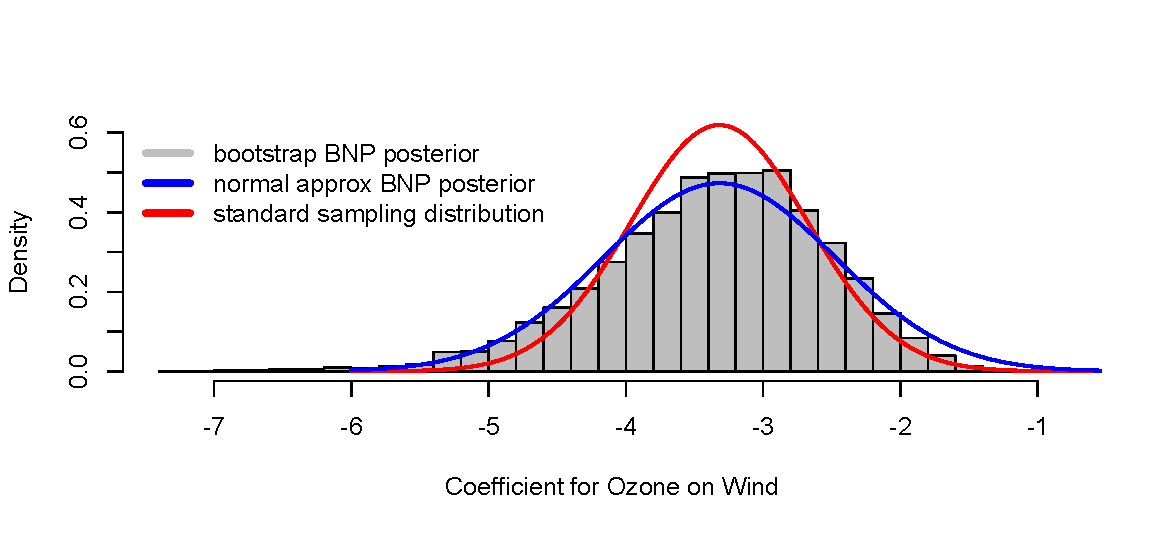
\includegraphics[width=\textwidth]{graphs/ozone}
\end{frame}

\begin{frame}[fragile]

{\footnotesize\nv
\begin{verbatim}
data(airquality); n <- nrow(airquality)
B <- 1000; beta <- vector(length=B)
for(b in 1:B){
  fit <- lm(Ozone ~., data=airquality, weights=rexp(n))
  beta[b] <- coef(fit)["Wind"] }
sampfit <- lm(Ozone ~ ., data=airquality)
coef <- summary(sampfit)$coef["Wind",1:2]
x <- as.matrix(cbind(1,na.omit(airquality)[,-1]))
xxi <- solve(crossprod(x))
sandwich <- xxi%*%t(x)%*%diag(sampfit$resid^2)%*%x%*%xxi
hist(beta, col=8, main="", 
  xlab="Coefficient for Ozone on Wind", 
  freq=FALSE,ylim=c(0,0.6),breaks=25)
grid <- seq(-6,5,length=500)
lines(grid, dnorm(grid,coef[1],coef[2]),col=2,lwd=2)
lines(grid, dnorm(grid,coef[1],sqrt(sandwich[3,3])),col=4,lwd=2)
legend("topleft",col=c(8,2),lwd=4, 
  legend=c("bootstrap BNP posterior",
           "normal approx BNP posterior",
           "standard sampling distribution"),bty="n")
\end{verbatim}
}

\end{frame}

\begin{frame}

{\nv \bf What is the blue line? } \\BB sampling is great, but analytic approximations are also useful.

\vskip .5cm
Consider a first-order Taylor series approximation,
\[
\bs{\tilde \beta} = [\bm{X}'\bm{X}]^{-1}\bm{X}'y + 
\nabla \bs{\beta}\big |_{\bs{\theta}=\bm{1}} (\bs{\theta} - \bm{1})
\]

We can derive {\it exact} posterior moments for $\bs{\tilde \beta}$ under $\theta_i \stackrel{iid}{\sim}\mathrm{Exp}(1)$.

\vskip .25cm
e.g., $\mr{var}(\bs{\tilde \beta}) \approx (\bm{X}^{\prime}\bm{X})^{-1}\bm{X}^{\prime}\mr{diag}(\bm{e})^2\bm{X}^{\prime}(\bm{X}^{\prime}\bm{X})^{-1}$, where $e_i  = y_i - \bm{x}_i'\bs{\hat\beta}$.

\vskip .25cm
This is the familiar Huber-White `Sandwich' variance formula.

\vskip .25cm{\gr \hfill
 See Lancaster 2003 or Poirier 2011.}

\end{frame}

\begin{frame}

{\bf{\gr Example:} User-Specific Behavior in Experiments}

\vskip .5cm
{\nv eBay runs lots of experiments:} they make changes to the marketplace (website) for random samples of users.

\vskip .5cm
Every experiment has response $y$ and treatment $d$ {\gr [0/1]}.

\vskip .5cm
We know $\bm{x}_i$ about user $i$.

\vskip .2cm
\begin{itemize}\gr
\item Their previous spend, items bought, items sold...
\item Page view counts, items watched, searches, ...
\item All of the above, broken out by product, fixed v. auction, ...
\end{itemize}

\vskip .25cm
$\bm{x}_i$ are  possible sources of heterogeneity. About 400 in our example.

\end{frame}

\begin{frame}

What is `heterogeneity in treatment effects'? {\gr(HTE)}

\vskip .5cm Different units {\gr [people, devices]} respond differently to some treatment you apply {\gr [change to website, marketing, policy]}.  

\vskip .5cm I imagine it exists.  

\vskip .5cm Can we accurately measure heterogeneity (index it on $\bm{x}$), \\~~ and how is this useful for decision making?

\end{frame}


\begin{frame}

In our illustrative example,
$d_i$ = bigger pictures in my eBay.

\vskip .25cm
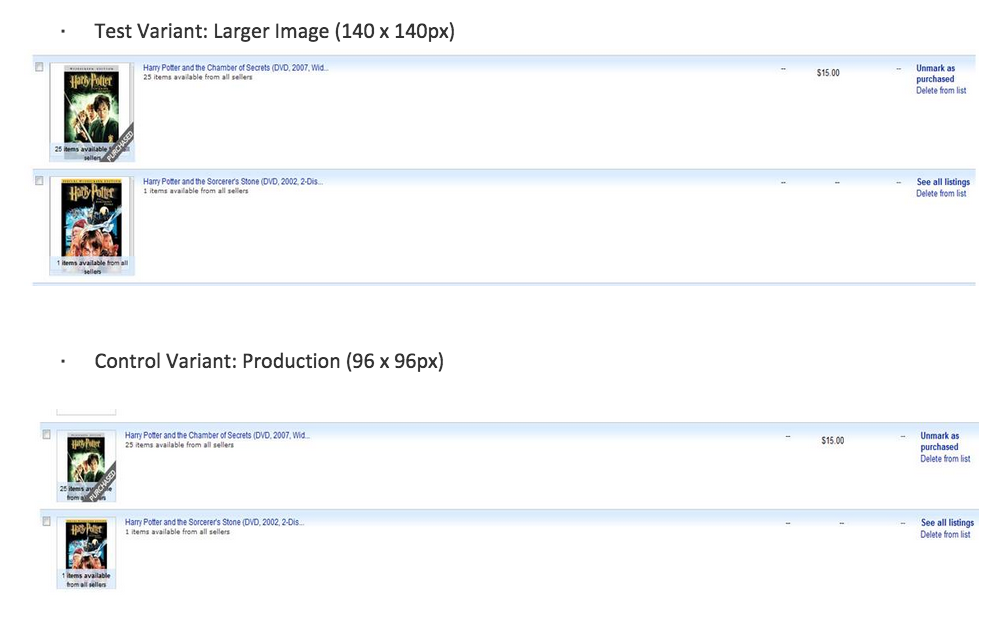
\includegraphics[width=4.5in]{graphs/userex}

21 million tracked visitors over 5 weeks, 2/3 in treatment.
\vskip -.5cm

\end{frame}

% \begin{frame}

% An `A/B' experiment
% \begin{itemize}
% \item Randomly expose users to control $\sf c$ or treatment $\sf t$.
% \item Calculate the mean for each, $\bar{y}_{\tt c}$ and $\bar{y}_{\tt t}$.
% \item The estimated `average treatment effect' is $\hat\gamma_{\mr{ate}} = \bar{y}_{\tt t} - \bar{y}_{\tt c}$, and it has variance
% \[
% \sigma^2_{ \mr{ate}}  = \frac{\mr{var}(\bm{y}_{\sf t})}{n_{\sf t}}
% + \frac{\mr{var}(\bm{y}_{\sf c})}{n_{\sf c}}
% \]
% \end{itemize}
% If $\hat\gamma_{\mr{ate}}/\sigma_{ \mr{ate}} > 2$ your stuff banks.

% \end{frame}


% \begin{frame}

% What about $\bm{x}$?


% \vskip .25cm
% Leads to $p=400$ covariates for each user, \\
% including `buying pattern factors'.
% \begin{itemize}
% \item very sparse.
% \item highly correlated with each other.
% \end{itemize}

% \vskip .25cm
% What can $\bm{x}$ tell us?

% \end{frame}

\begin{frame}

{\theme a statistic we care about ...}

\vskip .25cm
Potential outcome: $\upsilon_{i}({\sf d})$ is $\approx$ \$ for user
$i$ under  ${\sf d}$.  

\vskip .05cm
We only ever get to see one of $\upsilon_{i}({\sf t})$ and $\upsilon_{i}({\sf c})$: `y'.

\vskip .25cm
We care about `$\bs{\gamma}$' from the {\it moment condition}
\[
\ds{E}\left[\bm{x}(\upsilon({\sf t}) - \upsilon({\sf c})-\bm{x}'\bs{\gamma})\right] = \bs{0} 
\]
This says $\bm{x}'\bs{\gamma}$ is uncorrelated with the treatment effect $\upsilon({\sf t}) - \upsilon({\sf c})$.

\vskip .25cm
An extra randomization condition impies
\[
\bs{\gamma} = 
\ds{E}\left[\bm{x}\bm{x}'\right]^{-1}
\bigg(\ds{E}[\bm{x}y | {\sf d} = {\sf t}] - \ds{E}[\bm{x}y|  {\sf d} = {\sf c}]\bigg)
\]
\vskip .2cm
since $\ds{E}[\bm{x}\upsilon({\sf d})] = \ds{E}[\bm{x}\upsilon({\sf d}) | d]$ for randomized control trial.

\end{frame}


\begin{frame}

{\theme approximate mean and variance ...}

\vskip .25cm
One can show that
\[
\ds{E}\bs{\gamma} \approx \bs{\hat \gamma} = n(\bm{X}'\bm{X})^{-1}
 \left(\frac{\bm{X}_{\sf t}'\bm{y}_{\sf t}}{n_{\sf t}} - 
 \frac{\bm{X}_{\sf c}'\bm{y}_{\sf c}}{n_{\sf c}}\right)
\]
and we have an approximate variance (not too messy) $\bs{\Sigma}_{\bs{\tilde\gamma}}$.


\vskip 1.5cm
\hfill Or you can bootstrap, but it takes a long time.
\end{frame}

\begin{frame}

e.g., coefficient on purchase within last-year vs an intercept:

\vskip .25cm
{\footnotesize\it
\gr million users:~~~~~~~~~~~~~~~7.45~~~~~~~~~~~~~~~~~~~~~~10.97~~~~~~~~~~~~~~~~~~~~~13.22}
\begin{center}
\vskip -.5cm
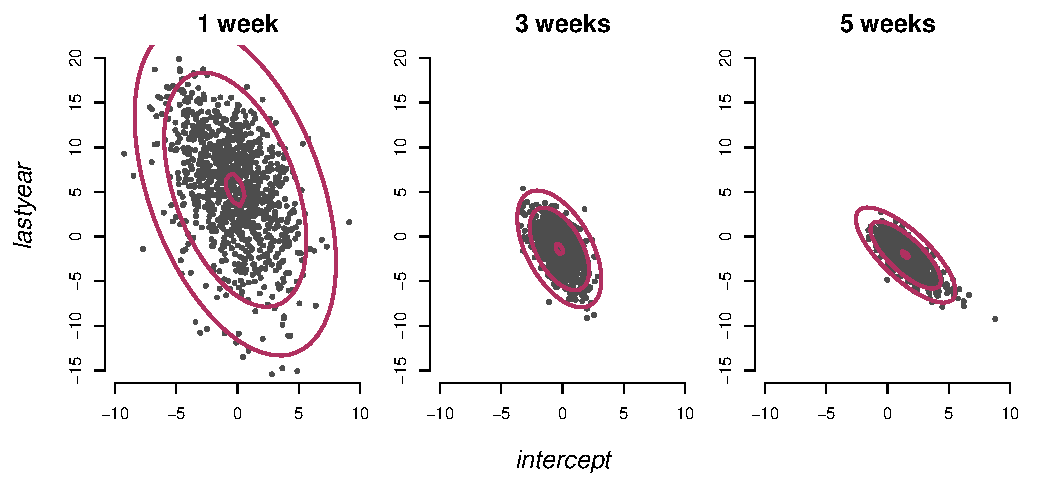
\includegraphics[width=.9\textwidth]{graphs/gammapost}
\end{center}

\vskip .25cm
{\gr Sample is from posterior, contours are normal approximation.}

{This is a statistic we care about}, even if the truth is nonlinear.

\vskip -.5cm
\end{frame}

\begin{frame}

{\theme Mining heterogeneity}

\vskip .5cm
We have 400 possible `directions' of heterogeneity in $\bs{\gamma}$.

\vskip .1cm Various levels of confidence in each, and they are highly correlated.


\vskip .5cm
Can we pick out a few that look promising for exploration?

\vskip .5cm
Be Bayesian: write down a {\it loss function} for what we decide to report, and choose the decision to minimize expected loss.

\end{frame}


\begin{frame}


\vskip .5cm
Say $\bs{\delta}$ is our `decided' vector of heterogenaity.  

\vskip .25cm
We want it to be mostly zero -- keep count $|\delta_j \neq 0|$ small.

\[
\ds{E}[\text{loss}] = \sum_i \frac{(\bm{x}_i\bs{\delta}-\bm{x}_i\bs{\hat\gamma})^2}{2n\mr{var}(\bm{x}_i\bs{\gamma})} + \lambda |\delta_j \neq 0|
\]
{\gr Penalty $\lambda>0$ is your `cost of complexity': it's like a squelch.}

\vskip .5cm{\theme 
Minimize to get answers `close' to  best, with closeness discounted by uncertainty about that best guess,  using only a few covariates. }

\end{frame}

\begin{frame}

That actual minimization is tough, but we can get very close.


\vskip .5cm
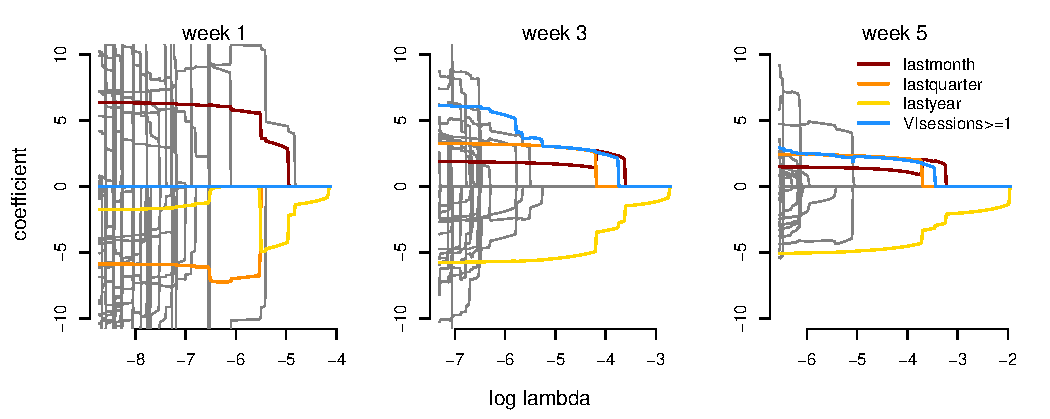
\includegraphics[width=1\textwidth]{graphs/sparsehighlights}

This shows $\bs{\delta}$ (vertical axis) as a function $\lambda$ (cost of complexity).

\vskip -.25cm
\end{frame}

\begin{frame}[fragile]

Slices of this path provide
representations of heterogenaity. 

\vskip .25cm
The best 3-factor model has treatment effects on capped GMB

\vspace{-.25cm}
\begin{semiverbatim}\nv
   newuser  lastmonth   lastyear       PC3   
      4.66       6.60       0.10      2.23  
\end{semiverbatim}

PC3 is big for sellers, viewers, and buyers of `unknown' items.  
\vskip .1cm
{\theme ~~~~Our `treasure hunters'!}

\vskip .25cm
Heterogenaity! Get 'em with bigger pictures!  


\end{frame}



\begin{frame}


{\bf {\theme Example 2:} Decision Trees are awesome}

\vskip .1cm 
They  learn non-linear response functions
\\ discover interactions between variables,
\\ and don't care about heteroskedasticity.

\vspace{-1cm}
\begin{adjustwidth}{-.3in}{}
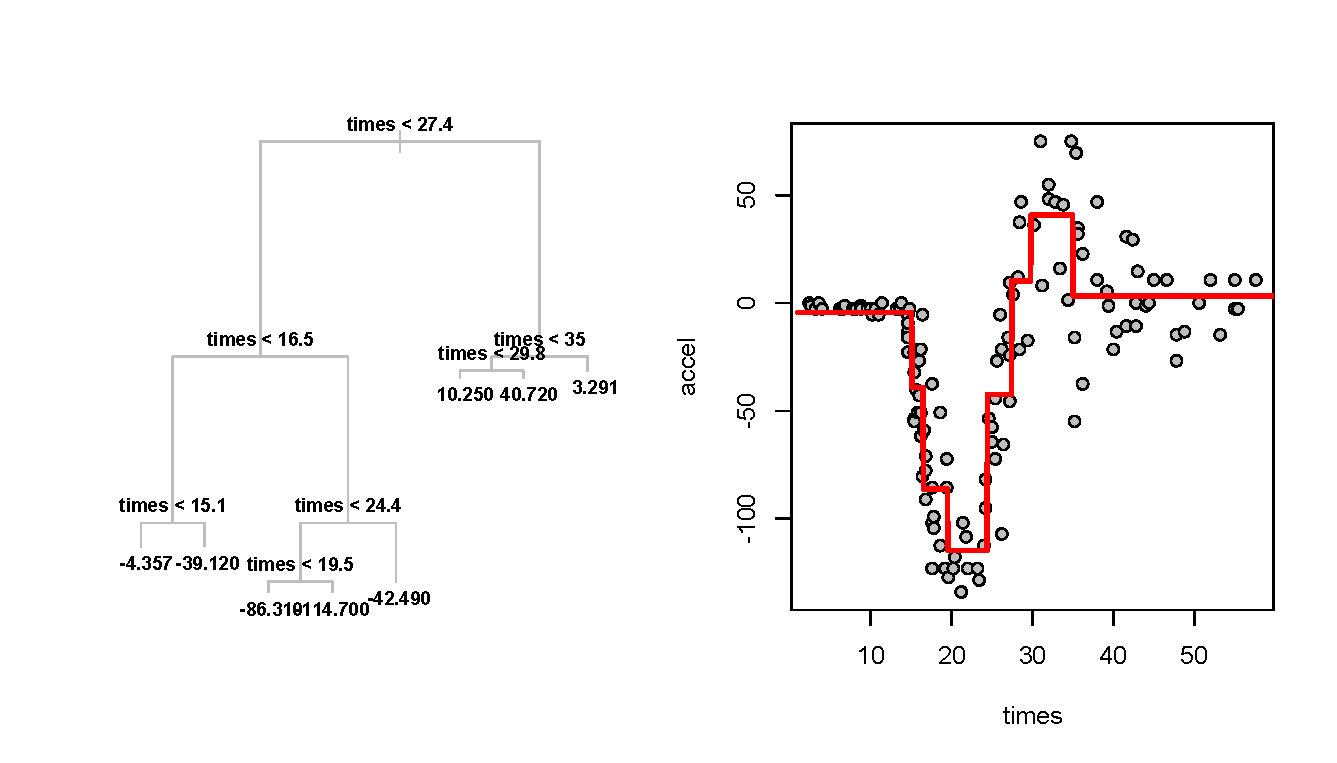
\includegraphics[width=4.6in]{../../bayesian-forest/graphs/MCtree}
\end{adjustwidth}

\vskip -.75cm
\end{frame}

\begin{frame}[fragile]


{\theme The CART tree is a statistic we care about.}

{\gr Imagine CART on the population: it would predict well.}

\vskip .25cm
{\sc Bayesian Forest}
\begin{algorithmic}
   \FOR{$b=1$ {\bfseries to} $B$}
   \STATE draw $\boldsymbol{\theta}^b \stackrel{iid}{\sim} \mathrm{Exp}(\mathbf{1})$
   \STATE run weighted-sample CART to get $\mathcal{T}_b = \mathcal{T}(\boldsymbol{\theta}^b)$
   \ENDFOR
\end{algorithmic}

\vskip .25cm\small 
~~~~~~~~~~~~~~~~~~~~~~~~{\it one tree~~~~~~~~~~~~~~~~~~~~~~~~~~~posterior mean}\\
~~~~~~~
\includegraphics[height=1.5in]{../../bayesian-forest/graphs/MCtreedraw}   
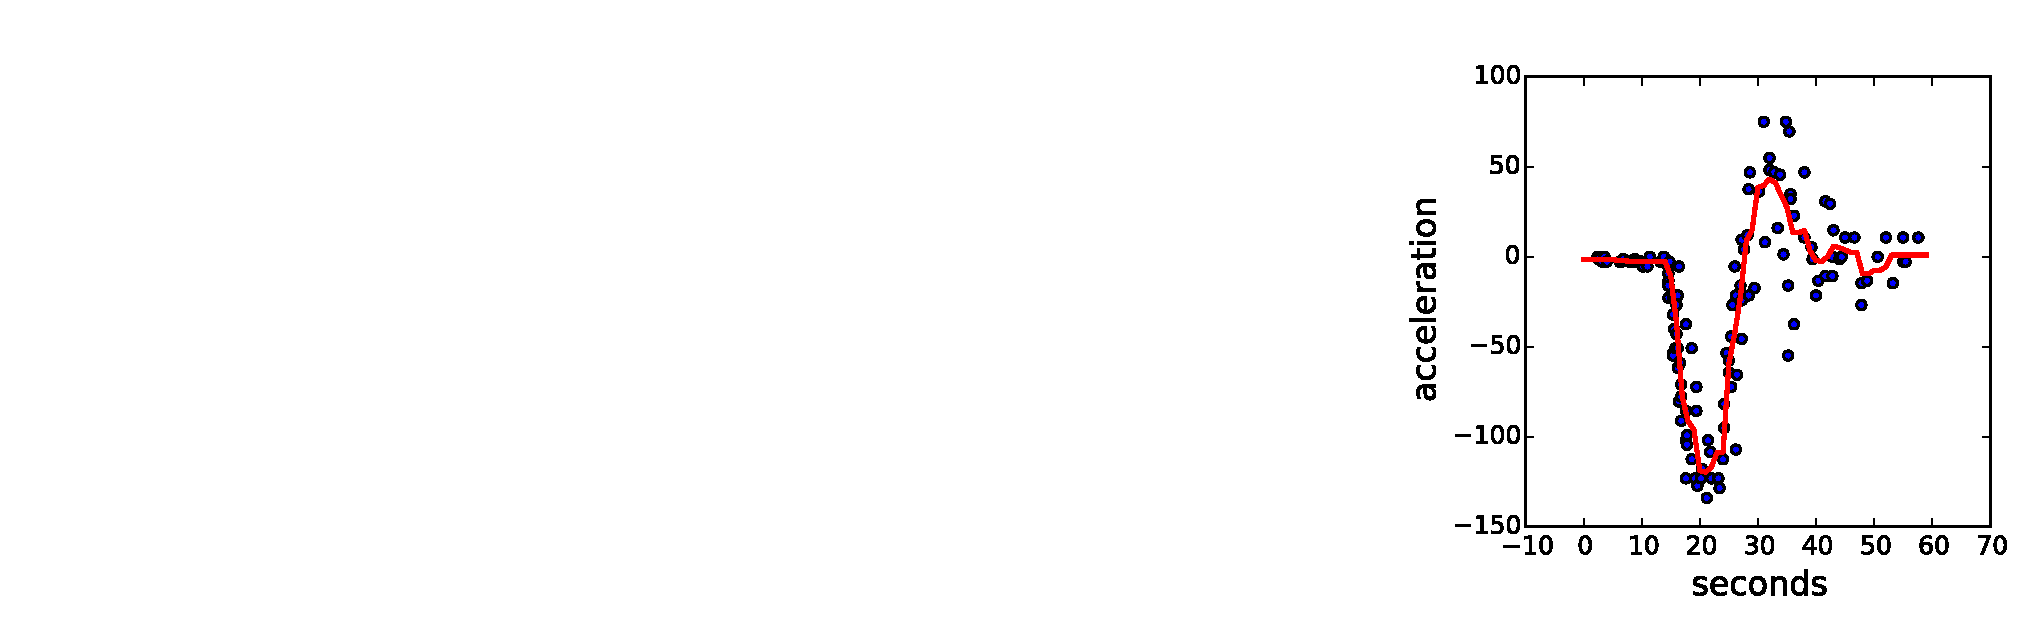
\includegraphics[height=1.5in]{../../bayesian-forest/graphs/MCbforest}   
\vskip -.5cm

\end{frame}



\begin{frame}

{\bf Theoretical trunk stability}

\vskip .5cm

Given forests as a posterior, 
we can start talking about {\it variance}.

\vskip .25cm
We are able to derive theoretically that the earliest structure in the tree -- {\theme the trunk} -- should be very stable for large samples.

\vskip .5cm
For the data at a given node, 
\begin{equation*}
\mathrm{p}\left(\text{optimal split matches sample CART}\right) \gtrsim 1 - \frac{p}{\sqrt{n}} e^{-n},
\end{equation*}
with $p$ split locations and $n$ observations.  

\vskip .5cm Things are pretty stable, until they aren't: as the tree grows,  node sizes get smaller and chance of a non-optimal split multiplies.

\end{frame}

\begin{frame}

{\bf California Housing Data}


\vskip .5cm

20k observations on median home prices in zip codes.

\vskip .5cm

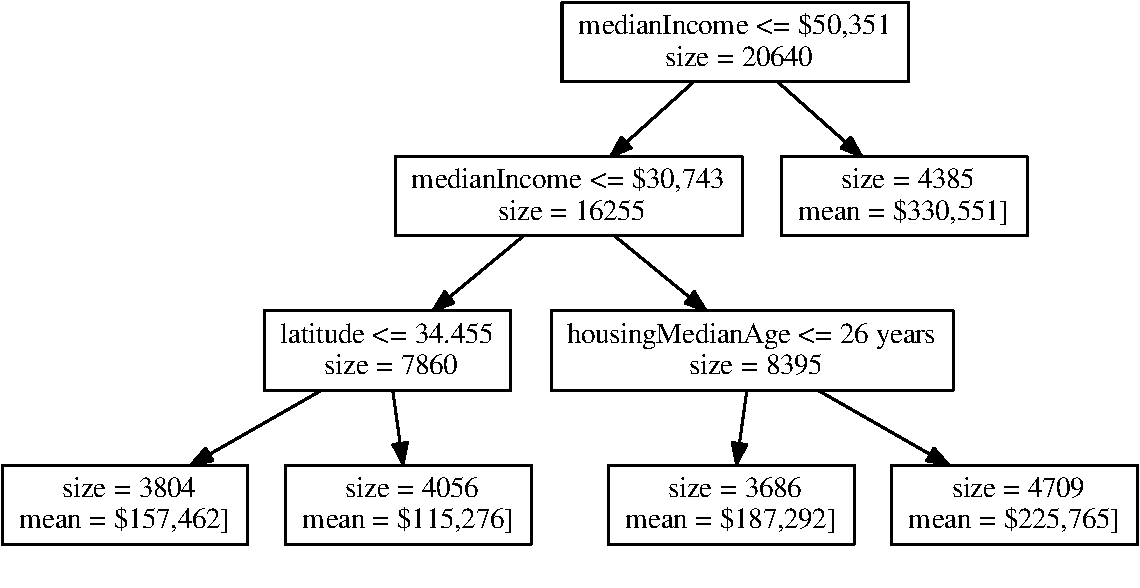
\includegraphics[width=\textwidth]{../../bayesian-forest/graphs/ca_trunk}

\vskip .5cm
\hfill Above is the trunk you get setting min-leaf-size of 3500.

\end{frame}

\begin{frame}

\begin{columns}

\begin{column}{2.15in}
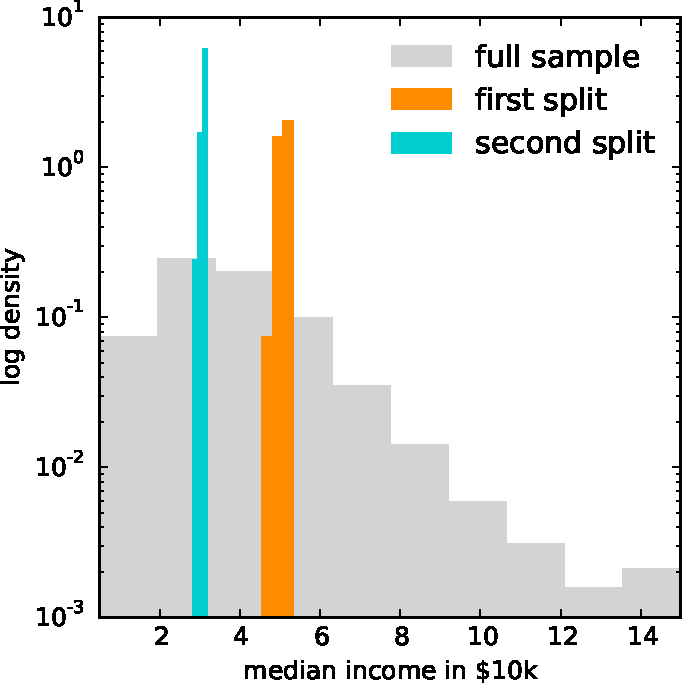
\includegraphics[width=2.5in]{../../bayesian-forest/graphs/ca_splits}
\end{column}

\begin{column}{2in}
\begin{itemize}
\item sample tree occurs 62\% \\of the time.  
\vskip .5cm
\item 90\% of  trees split on income twice, \\and then latitude. 

\vskip .5cm
\item 100\% of trees have 1st 2 splits on median income.  
\end{itemize}
\end{column}

\end{columns}


\vskip 1cm
~~~~Empirically and theoretically: trees are stable, at the trunk.
\vskip -1cm

\end{frame}

\begin{frame}


Forests are expensive when data is too big to fit in memory.

\vskip .2cm
Subsampling forests 
lead to a big drop in performance.

\vskip .2cm
{But wait:}  if the trunks are stable, can we just fit that once and then fit forests at each branch?  {\nv Yes!}

\vskip .5cm
{\bf Empirical Bayesian Forests ({\theme EBF}):}

\vskip .25cm
\begin{itemize}
\item fit a single tree to a shallow {\nv trunk}.  
\item Use this as a mapper to direct full data to each {\nv branch}.  
\item Fit a full  forest on the smaller branch datasets.
\end{itemize}

\vskip .25cm
This is classic Empirical Bayes: fix higher levels in a {\it hierarchical model}, and direct your machinery\texttt{+}data at learning the hard bits.

\end{frame}

\begin{frame}


Since the trunks are all the same for each tree in a full forest,
our EBF looks nearly the same at a fraction of computational cost.

\begin{center}
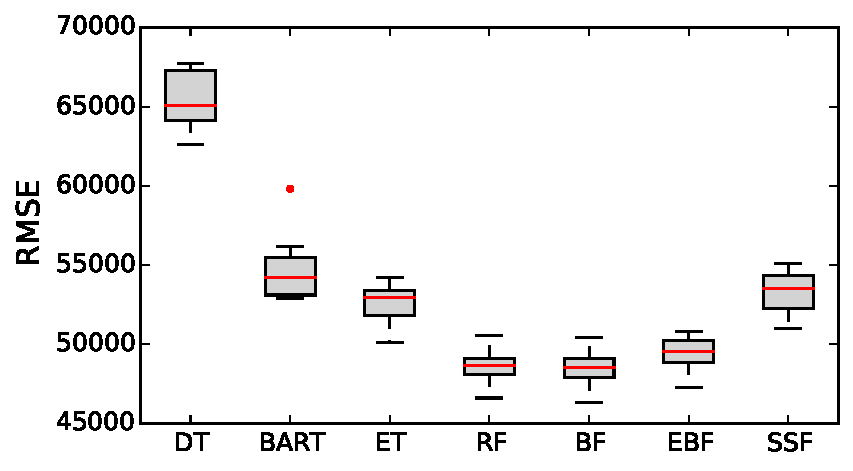
\includegraphics[width=.85\textwidth]{../../bayesian-forest/graphs/ca_rmse}
\end{center}

Here EBF and BF give nearly the same results.  {\it SSF does not.}


\end{frame}


\begin{frame}


{\bf \theme EBFs at EBay: \bk predicting Bad Buyer Experiences}

\vskip .5cm
A BBE could be receiving something that is `significantly not as described',
or shipping delays, or any of many other problems.

\vskip .5cm
The models are updated frequently, and  information\\ about $\mathrm{p}(\text{BBE})$
is an input to search rankings  and more.

\vskip .5cm The best thing to improve predictions is more data.  \\With millions of daily transactions, there's little limit on data.

\end{frame}

\begin{frame}

{\bf EBFs at EBay}

\vskip .5cm
Random forest runs take too long on full data.

\vskip .25cm
Subsampling led to a noticeable and big drop in performance.

\vskip .5cm
So: EBFs!
\begin{itemize}
\item trunk can be fit in distribution using Spark \texttt{MLLib}.
\item this trunk  acts as a sorting function to map observations \\to 
separate locations corresponding to each branch.
\item Forests are then fit on a machine for each branch.  
\end{itemize}



\end{frame}

\begin{frame}

{\bf EBFs at EBay}

\vskip .5cm

On 12 million transactions,  EBF with 32 branches yields a\\ 1.3\% drop in misclassification over the SSF alternatives.  

\vskip .5cm 
Putting it into production requires some careful engineering, \\but this really is a very simple algorithm.  {\theme Big gain, little pain.} 

\vskip .5cm
A key point:  EBFs are not inherently `better' than forests fit to all of the data.  But EBFs can be fit to {\nv more data} in less time.

\end{frame}


\begin{frame}

\vskip .5cm
{\bf Efficient Big Data analysis}

\vskip .25cm
To cut computation without hurting performance, we need to think about what portions of the `model' are {\theme hard} or {\nv easy} to learn.

\vskip .25cm
Once we figure this out,  we can use a little bit of the data to\\ learn the easy stuff and direct our full data at the hard stuff.

\vskip .25cm
I believe that this is the future for Big Data.

\vskip .75cm
{\bf Big Data and distribution free BNP}

\vskip .25cm I think about BNP as a way to analyze (and improve) algorithms.  

Decouple  action/prediction from the full generative process model.

\vskip 1cm
\hfill \huge \theme \bf thanks!

\end{frame}



\end{document}






























